\documentclass{article}

% Language setting
% Replace `english' with e.g. `spanish' to change the document language
\usepackage[english]{babel}

% Set page size and margins
% Replace `letterpaper' with `a4paper' for UK/EU standard size
\usepackage[
    a4paper,
    top=2cm,
    bottom=2cm,
    left=3cm,
    right=3cm
]{geometry}

% Useful packages
\usepackage{amsmath}
\usepackage{graphicx}
\usepackage[colorlinks=true, allcolors=blue]{hyperref}
\usepackage{tikz}
\usetikzlibrary{positioning, arrows.meta, shapes.geometric, fit}

\title{Smart visual alarm system \\
\large An edge TinyML-Based visual monitoring system using ESP32-S3-EYE and Raspberry Pi}
\author{Stefano Murtas}

\begin{document}
\maketitle

\begin{abstract}
Your abstract.
\end{abstract}

\section{Introduction}

The Internet of Things (IoT) enables physical devices to sense their
environment, process information, communicate with other devices and
services, and trigger actions according to the observed conditions.
An IoT system can therefore combine sensing, computation, communication,
and application-level services to transform observations of the physical
world into useful information and actions.

Visual monitoring represents a particularly challenging IoT application.
Compared with conventional sensors that produce relatively small amounts
of data, cameras continuously generate images containing a much larger
amount of information. A simple solution would be to transmit the acquired
images to a local server or cloud infrastructure and perform the required
computer vision processing remotely. However, this approach increases
network traffic, requires an external processing infrastructure, and
transmits visual information even when the observed scene does not contain
any relevant event.

An alternative approach is to move part of the computation closer to the
source of the data. In an edge computing architecture, information can be
processed locally before being transmitted to other components of the IoT
system. When machine learning inference is executed directly on
resource-constrained microcontrollers, this approach leads to Tiny Machine
Learning (TinyML).

TinyML combines machine learning with embedded computing under strict
constraints in terms of memory, storage, computational capability, latency,
and energy consumption. Consequently, developing a TinyML application
requires considering not only the predictive performance of a machine
learning model, but also whether the model can be efficiently executed on
the target embedded platform.

This paradigm is particularly suitable for an intelligent visual monitoring
system: rather than using the camera as a passive sensor that continuously
transmits images for remote analysis, the embedded device can locally
interpret the acquired visual information and communicate only when a
relevant event is detected.

This concept represents the starting point of the \emph{Smart visual alarm
system} developed in this project.

\section{System Overview}

\subsection{Use Case and Target Scenario}

The target scenario of this project is the monitoring of a mountain house environment. In this context, people and animals may pass near the entrance or in the surrounding outdoor area, also during evening or night hours. The objective is to develop a smart visual alarm system able to detect relevant visual events and notify the user remotely.

Unlike a generic indoor people detection system, this project focuses on a more specific real-world scenario. The monitored area is expected to contain different types of situations: an empty scene, the presence of a person, or the presence of a generic animal. The goal is not to recognize the animal species, since this would require a larger and more complex dataset, but to distinguish between the main classes that are relevant for the alarm system.

The camera is positioned near the entrance of the house, with a clear view
of the monitored outdoor area. The camera observes the scene through a
window protected by metal bars, which are therefore permanently visible
in the foreground of the acquired images. These elements can partially
occlude people or animals and make visual classification more challenging,
especially when a subject is located behind or close to the bars.

The installation environment also includes an automatic light that is
activated by motion. This provides additional illumination under low-light
conditions without requiring an infrared camera, although night-time visual
classification is not considered a separate machine learning task in this
project.

The proposed use case is therefore based on three target classes:
\begin{itemize}
    \item \textbf{Empty}: no relevant subject is visible in the monitored area;
    \item \textbf{Person}: at least one person is visible in the scene;
    \item \textbf{Animal}: at least one animal is visible in the scene,
without distinguishing its species.
\end{itemize}

When the system identifies a \textit{person} or an \textit{animal}, the
prediction confidence is evaluated before generating an alarm. In the final
implementation, an application-level confidence threshold of 0.85 (85\%) is used:
only detections with a confidence equal to or greater than this threshold
are propagated through the IoT notification pipeline. Lower-confidence
predictions remain visible in the device logs for diagnostic purposes but
do not generate an external alert.

When the alert condition is satisfied, the captured image is transferred
from the ESP32-S3-EYE to the Raspberry Pi through HTTP, while the detection
event is published through MQTT. The event is subsequently processed using
Node-RED and a Telegram notification containing the captured image is sent
to the user. The resulting use case therefore combines local TinyML
inference with event-driven IoT communication, allowing both the visual
classification behaviour and the complete notification pipeline to be
evaluated in a real monitoring environment.

\subsection{General System Architecture}
\label{subsec:general-architecture}

The overall architecture of the Smart Visual Alarm System is shown in
Figure~\ref{fig:system_architecture}. The system is organized around an
ESP32-S3-EYE edge node, a Raspberry Pi gateway, an MQTT communication layer,
Node-RED, and a Telegram notification service.

The ESP32-S3-EYE performs image acquisition, preprocessing, TinyML inference,
and the application-level alert decision locally. When a relevant event is
detected, the captured image is transferred to the Raspberry Pi through HTTP,
while the detection event is published through MQTT. The Raspberry Pi then
handles the downstream IoT integration, and Node-RED processes the event flow
that ultimately triggers the Telegram notification.

This architecture separates local visual intelligence from the communication
and notification infrastructure, following an edge-oriented and event-driven
design.

\begin{figure}[htbp]
\centering
\resizebox{0.98\textwidth}{!}{
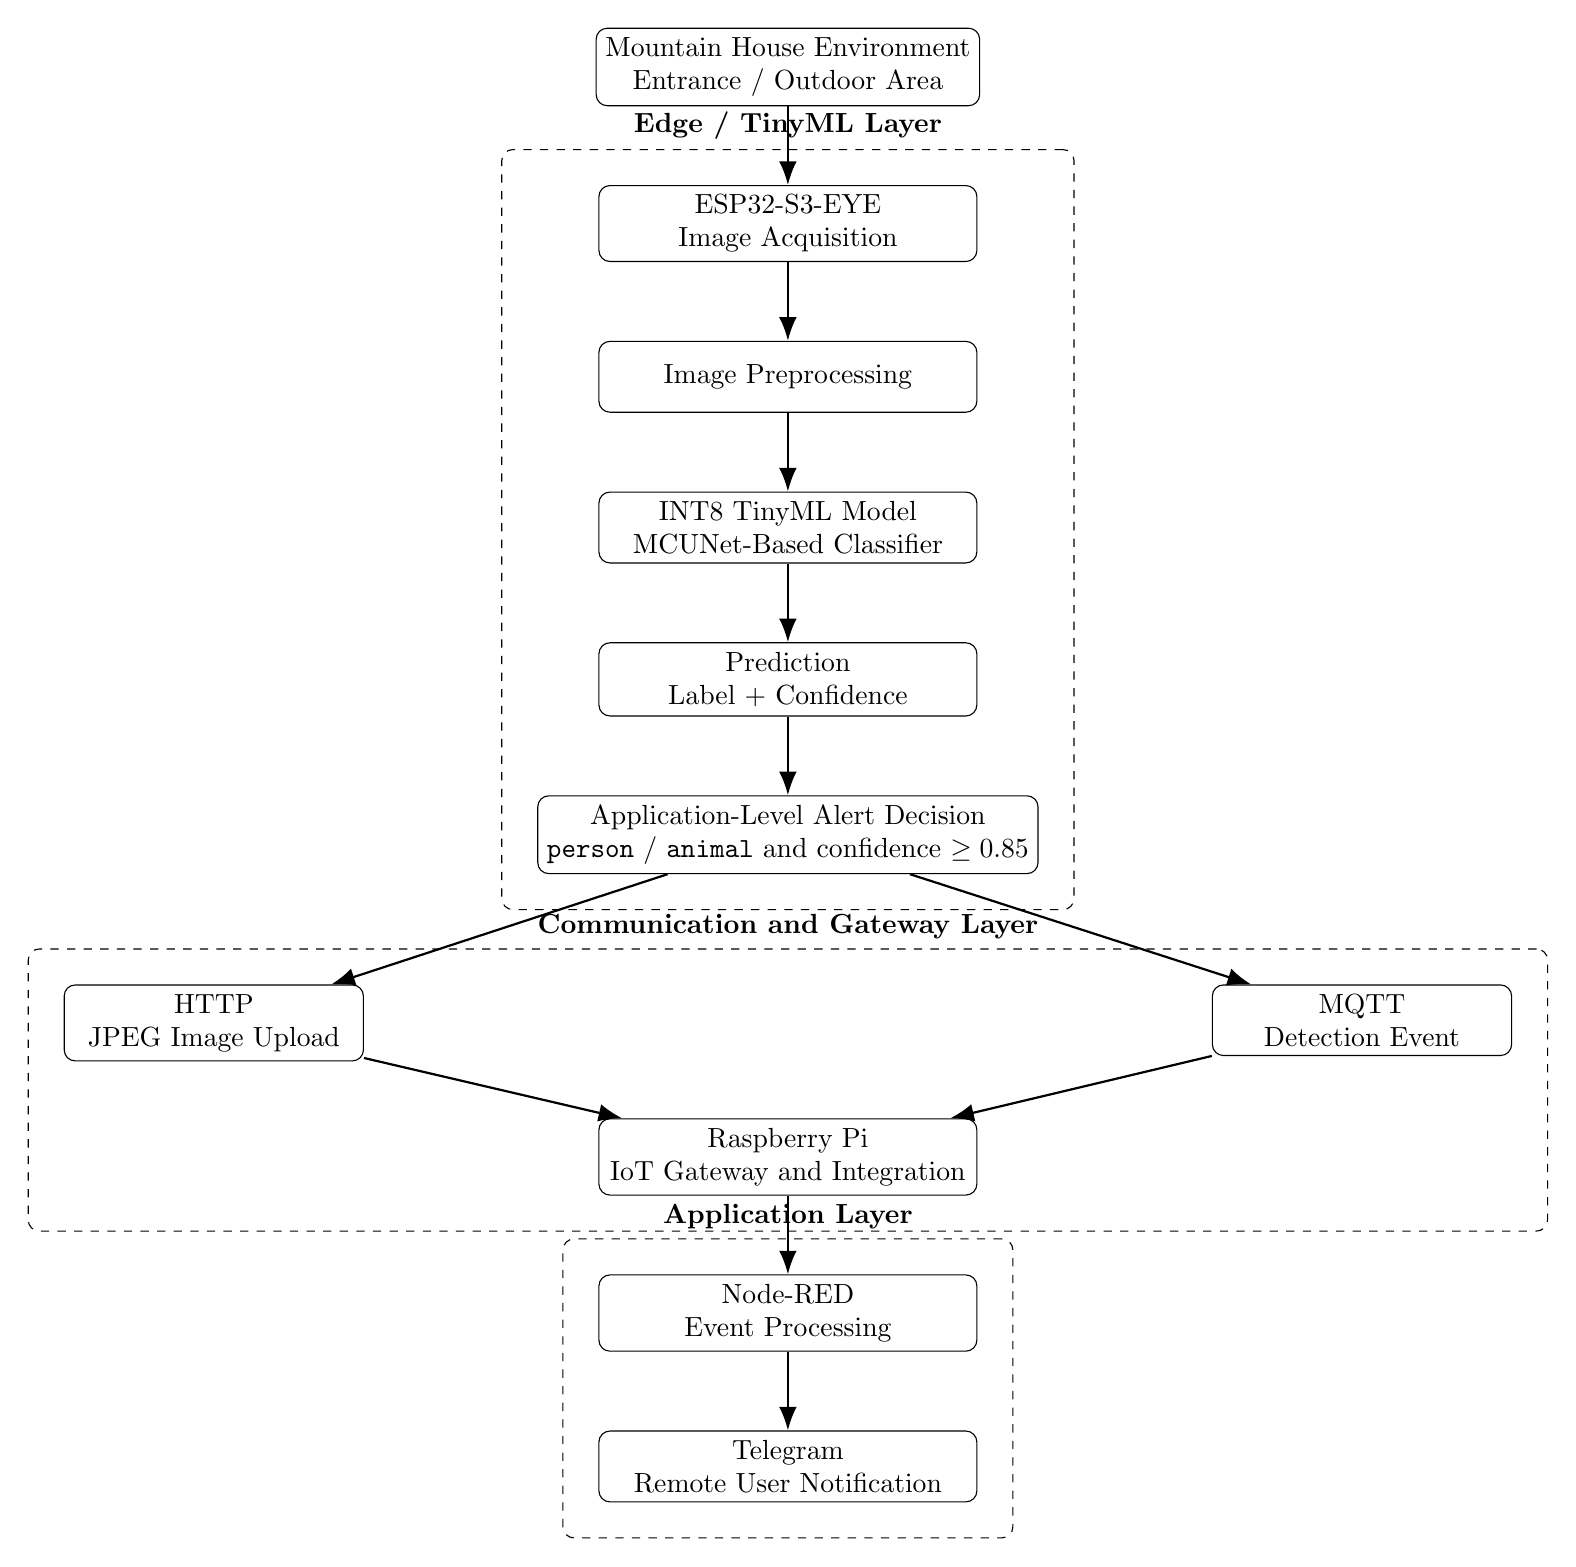
\begin{tikzpicture}[
    node distance=1.0cm and 1.8cm,
    block/.style={
        rectangle,
        rounded corners,
        draw,
        align=center,
        minimum width=4.8cm,
        minimum height=0.9cm
    },
    smallblock/.style={
        rectangle,
        rounded corners,
        draw,
        align=center,
        minimum width=3.8cm,
        minimum height=0.8cm
    },
    layer/.style={
        rectangle,
        rounded corners,
        draw,
        dashed,
        inner sep=0.45cm
    },
    arrow/.style={
        -{Latex[length=3mm]},
        thick
    }
]

% ------------------------------------------------------------------
% EDGE LAYER
% ------------------------------------------------------------------

\node[block] (scene) {Mountain House Environment\\Entrance / Outdoor Area};

\node[block, below=of scene] (camera)
{ESP32-S3-EYE\\Image Acquisition};

\node[block, below=of camera] (preprocessing)
{Image Preprocessing};

\node[block, below=of preprocessing] (model)
{INT8 TinyML Model\\MCUNet-Based Classifier};

\node[block, below=of model] (prediction)
{Prediction\\Label + Confidence};

\node[block, below=of prediction] (decision)
{Application-Level Alert Decision\\
\texttt{person} / \texttt{animal} and confidence $\geq 0.85$};

% ------------------------------------------------------------------
% COMMUNICATION / GATEWAY LAYER
% ------------------------------------------------------------------

\node[smallblock, below left=1.4cm and 2.2cm of decision] (http)
{HTTP\\JPEG Image Upload};

\node[smallblock, below right=1.4cm and 2.2cm of decision] (mqtt)
{MQTT\\Detection Event};

\node[block, below=3.1cm of decision] (raspberry)
{Raspberry Pi\\IoT Gateway and Integration};

% ------------------------------------------------------------------
% APPLICATION LAYER
% ------------------------------------------------------------------

\node[block, below=of raspberry] (nodered)
{Node-RED\\Event Processing};

\node[block, below=of nodered] (telegram)
{Telegram\\Remote User Notification};

% ------------------------------------------------------------------
% CONNECTIONS
% ------------------------------------------------------------------

\draw[arrow] (scene) -- (camera);
\draw[arrow] (camera) -- (preprocessing);
\draw[arrow] (preprocessing) -- (model);
\draw[arrow] (model) -- (prediction);
\draw[arrow] (prediction) -- (decision);

\draw[arrow] (decision) -- (http);
\draw[arrow] (decision) -- (mqtt);

\draw[arrow] (http) -- (raspberry);
\draw[arrow] (mqtt) -- (raspberry);

\draw[arrow] (raspberry) -- (nodered);
\draw[arrow] (nodered) -- (telegram);

% ------------------------------------------------------------------
% LAYER BOXES
% ------------------------------------------------------------------

\node[layer, fit=(camera)(preprocessing)(model)(prediction)(decision),
      label={[font=\bfseries]above:Edge / TinyML Layer}] (edgebox) {};

\node[layer, fit=(http)(mqtt)(raspberry),
      label={[font=\bfseries]above:Communication and Gateway Layer}] (commbox) {};

\node[layer, fit=(nodered)(telegram),
      label={[font=\bfseries]above:Application Layer}] (appbox) {};

\end{tikzpicture}
}
\caption{Layered architecture of the Smart Visual Alarm System. The ESP32-S3-EYE
performs local image acquisition, preprocessing, TinyML inference and alert
decision at the edge. Relevant detections trigger HTTP image transfer and MQTT
event publication towards the Raspberry Pi, while Node-RED manages the
application workflow and generates the Telegram notification.}
\label{fig:system_architecture}
\end{figure}

\subsection{Hardware Components}
\label{subsec:hardware-components}

The hardware architecture is based on two main devices: the ESP32-S3-EYE
and a Raspberry Pi. The two platforms have complementary roles within the
system.

The ESP32-S3-EYE acts as the intelligent sensing node. It acquires images
from the monitored environment and performs the complete local inference
pipeline, including image preprocessing, execution of the TinyML model, and
evaluation of the resulting prediction. Its role is therefore not limited
to image acquisition: the device is responsible for deciding whether the
observed scene contains a relevant event before any alert is propagated
through the network.

The Raspberry Pi acts as the local gateway and integration platform. It
provides the services required to receive images from the ESP32-S3-EYE,
manage MQTT-based event communication, execute the Node-RED workflow, and
support the final Telegram notification process. Compared with the
microcontroller, the Raspberry Pi offers substantially greater computing,
storage, and networking capabilities, making it suitable for the
communication and application-level components that do not need to execute
directly on the embedded sensing node.

This division of responsibilities reflects the edge-oriented design of the
system: latency-sensitive visual inference is performed directly on the
ESP32-S3-EYE, while higher-level communication and integration tasks are
delegated to the Raspberry Pi.

\begin{figure}
\centering
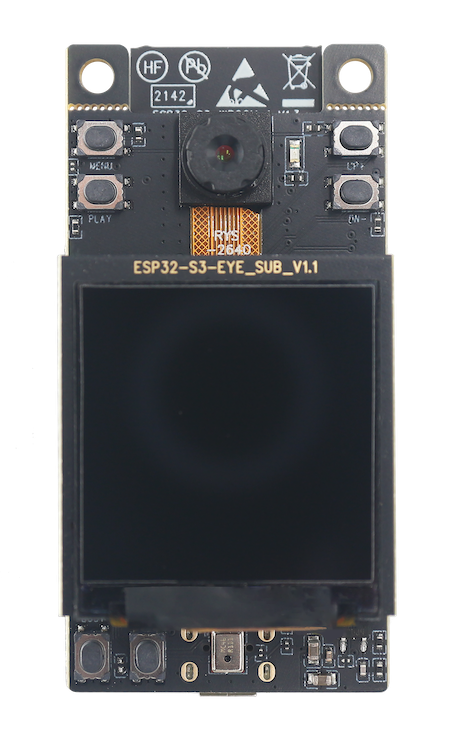
\includegraphics[width=0.25\linewidth]{ESP32-S3-EYE-isometric.png}
\caption{\label{fig:esp32_s3_eye}ESP32-S3-EYE board used for image acquisition and visual classification in the proposed smart visual alarm system.}
\end{figure}

\subsection{Software Components}
\label{subsec:software-components}

The software architecture of the Smart visual alarm system combines
embedded development, machine learning, communication protocols, and
flow-based IoT integration. Different software components are used at
different stages of the project, from neural network development and
deployment to the execution of the final notification pipeline.

On the embedded side, the ESP32-S3-EYE firmware is developed using
ESP-IDF. The firmware integrates camera acquisition, image preprocessing,
execution of the deployed TinyML model, application-level decision logic,
Wi-Fi connectivity, HTTP communication, and MQTT event publication.

The machine learning development pipeline is implemented in Python using
PyTorch. It includes dataset loading and preprocessing, model definition,
training, validation, and evaluation. After training, the selected model is
converted and quantized for deployment on the ESP32-S3-EYE, where inference
is performed locally using the Espressif embedded machine learning
infrastructure.

On the Raspberry Pi, the software stack provides the services required to
receive images and process alarm events. MQTT is used for lightweight
event communication, while HTTP is used for image transfer. Node-RED
orchestrates the downstream event flow and integrates the detection events
with Telegram, which provides the final remote notification to the user.

The resulting software stack therefore connects two distinct domains:
the machine learning pipeline used to develop and optimize the classifier,
and the IoT runtime infrastructure used to transform an on-device inference
result into a remote notification.

\section{Dataset Acquisition and Preparation}
\label{sec:dataset}

\subsection{Data Collection}
\label{subsec:data-collection}

A dedicated dataset was created for the development of the visual
classification model. The images were collected directly from the
ESP32-S3-EYE installed in the target monitoring environment, rather than
relying exclusively on an existing public dataset. This approach was chosen
to make the training data representative of the visual conditions that the
deployed system would encounter.

The camera was configured to acquire images of the entrance and surrounding
outdoor area of the mountain house. As a consequence, the collected images
share the same viewpoint and contain environmental characteristics that are
specific to the final deployment scenario, including the background,
illumination variations, subject distance, and the metal bars located in
front of the camera. These characteristics are particularly relevant because
they directly affect the visual information available to the classifier.

During the initial acquisition phase, images were periodically captured by
the ESP32-S3-EYE and transferred through the local network to the Raspberry
Pi, where they were stored for subsequent dataset preparation. At this stage,
the objective was to collect raw observations of the real environment before
performing manual classification into the three target classes:
\texttt{empty}, \texttt{person}, and \texttt{animal}.

Collecting the dataset in the actual deployment environment improves its
relevance to the target application, but also introduces an important
limitation: naturally occurring events are not equally frequent. Empty
scenes were significantly more common than images containing people and,
especially, animals. This class imbalance became one of the main challenges
of the dataset preparation process and required additional processing steps,
as discussed in the following subsections.
\subsection{Manual Labelling}
\label{subsec:manual-labelling}

After the acquisition phase, the collected images had to be manually
inspected and assigned to the correct target class. A dedicated Python
script, \texttt{label\_dataset.py}, was developed to support this process
and to create a consistently labelled dataset for model training.

The script displays the collected images sequentially and allows the user
to assign each image to one of the three classes: \texttt{empty},
\texttt{person}, or \texttt{animal}. Images that are corrupted, ambiguous,
or otherwise unsuitable for training can instead be assigned to a separate
\texttt{rejected} category. According to the selected label, the image is
automatically moved to the corresponding class directory.

Manual inspection was particularly important in this project because the
images were collected automatically from a real outdoor environment.
Consequently, not every acquired frame necessarily provided a clear and
useful training example. The labelling stage therefore served both to
associate each image with its ground-truth class and to perform an initial
quality-control step before training the neural networks.

The dataset directory structure was subsequently reorganized during the
development of the project. Therefore, the intermediate directory structure
used during the initial acquisition and labelling phases does not correspond
exactly to the final organization of the repository.

\subsection{Dataset Challenges and Class Imbalance}
\subsection{Data Augmentation}
\subsection{Dataset Split}

\section{GitHub Repository}

You can find the whole project at \url{https://github.com/smurtas/Smart-Visual-Alarm-System.git}.

\bibliographystyle{alpha}
\bibliography{sample}

\end{document}
